\documentclass[12pt]{article}

\usepackage[utf8]{inputenc}
\usepackage[T1]{fontenc}
\usepackage[top=2cm, bottom=3cm, left=3cm, right=3cm]{geometry}
\usepackage{url}
\usepackage{graphicx}
\title{Chabi Protocole}
\author{
  Cecilia BITOUT, Krimo HAMADI, Pin WANG, \\
  Jérôme SKODA et Joaquim LEFRANC
}

\date{2017}

\begin{document}
\fontfamily{cmr}
\maketitle

\newcommand{\separator}{\#\#}

\section{Adresse IP et port}

\begin{itemize}
  \item~Le port TCP utilisé est le 1027
  \item~IP UDP Multicast: 224.4.4.4
  \item~Port UDP Multicast : 4444
\end{itemize}


\section{Fonctionnement}

\subsection{Connexion}

La connexion au serveur d'annonce s'effecture en TCP sur le port 1027.

Après la connexion TCP, le serveur envois au client un message de type [WELC].

Le client doit alors s'enregistrer en envoyant la commande [NEWC]

Si l'opperation d'enregistrement du client s'est bien effectué alors le serveur renvois un [ACKC] au client et de la liste des annonces disponible [LIST\separator{}n\_annonce][ANNO][ANNO]...[ANNO]


\subsection{Ajout d'annonce}

Un client enregistré peut ajouter une annonce en envoyant un [ANNO\separator{}annonce\_id\separator{}src\_annonce\separator{}titre\_annonce\separator{}contenu\_annonce\separator{}prix] avec les argument annonce\_id et src\_annonce à 0 au serveur.


\subsection{Récupération des annonces}

Un client enregistré peut récuprer les annonce en envoyant un message [LIST] au serveur, le serveur répond avec un [LIST\separator{}n\_annonce][ANNO][ANNO]...[ANNO]

\subsection{Répondre à une annonce}

Un client enregistré peut repondre à une annonce en envoyant un message [MESS\separator{}id\_src\separator{}id\_dst\separator{}client\_message] à l'annonceur.

L'annonceur peux repondre en utilisant le même message en inversant id\_src et id\_dst.



\subsection{Suppression d'annonces}

Un client enregistré peut supprimé une annonce en envoyant [DELETE\separator{}id\_annonce]


\subsection{Déconnexion}

Un client enregistré peut se déconnecter en envoyant [BYE] au serveur, ces annonce devienne alors obsolete.

\section{Format des messages}


Le premier mot d'un message est un préfix indiquant le type de message, ces préfix sont conventionnelement écrient en majuscule.

Exemple: "ANNO, LIST, BYE" sont des préfix

Certain message contienne des arguments. Chacun de ces arguments sont séparé par deux \separator{} (ASCII 35),
il est interdit à un argument de contenir deux \separator{} à la suite.

Exemple:

[ANNO\separator{}451\separator{}124\separator{}salade\separator{}Une belle salade toute verte!\separator{}12.10]

Sera un message avec le prefix "ANNO"
Ces arguments seront:
\begin{itemize}
  \item~451
  \item~124
  \item~salade
  \item~"Une belle salade toute verte!"
  \item~12.10
\end{itemize}

\section{Liste des messages}

\begin{itemize}
  \item~[BYE]  Déconnexion d'un client
  \item~[ANNO\separator{}annonce\_id\separator{}src\_annonce\separator{}titre\_annonce\separator{}contenu\_annonce\separator{}prix]
  \begin{itemize}
    \item id\_annonce: <int>  id unique de l'annonce (à 0 s'il s'agit d'une création d'annonce)
    \item src\_annonce: <int> id unique de l'annonceur (à 0 s'il s'agit d'une création d'annonce)
    \item annonce\_titre : <string> titre
    \item annonce\_contenu : <string> contenu
    \item annonce\_prix : <double> prix
  \end{itemize}
  \item~[LIST n\_annonce] : Requête de liste d'annonce d'un client
  \begin{itemize}
    \item n\_annonce: <int> nombre d'annonce
  \end{itemize}
  \item~[MESS\separator{}id\_src\separator{}id\_dst\separator{}client\_message]
  \begin{itemize}
    \item id\_src: <int> id unique du client source
    \item id\_dst: <int> id unique du client destinataire
    \item client\_message : <string> message
  \end{itemize}
  \item~[DELETE\separator{}id\_annonce] : Reuqête de suppresion d'annonce d'un client
\end{itemize}


\section{Diagramme de connexion au serveur}

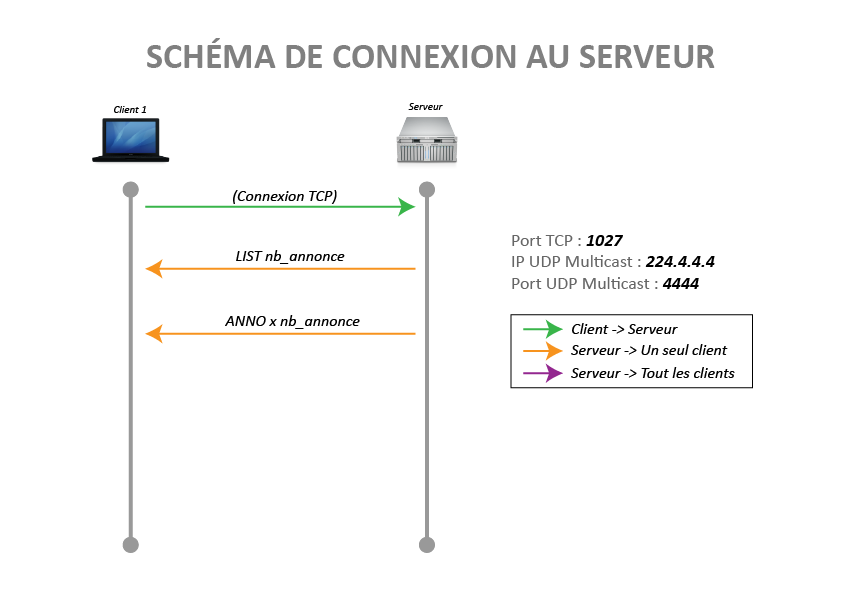
\includegraphics[width=\textwidth]{rendu1/Protocole_Connection.png}

\section{Diagramme des opérations}

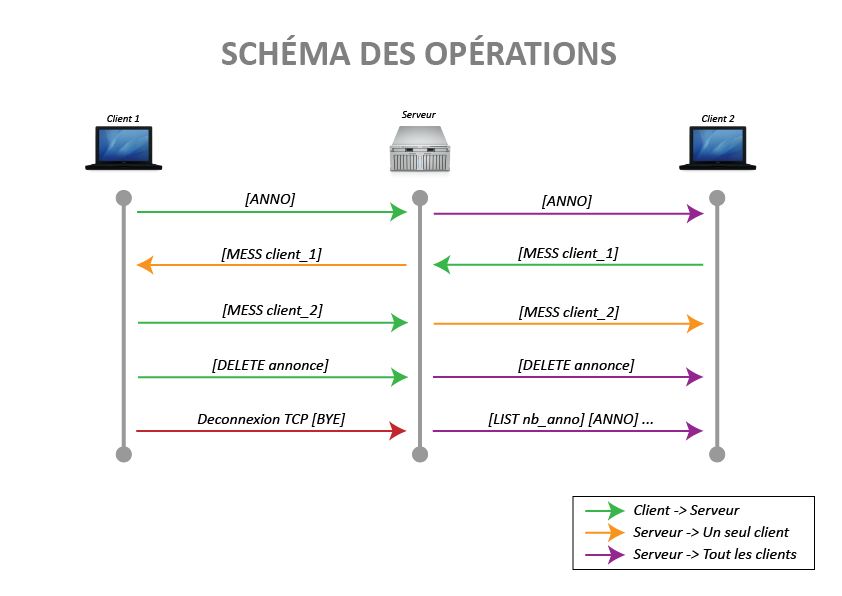
\includegraphics[width=\textwidth]{rendu1/Protocole_Operations.png}


\end{document}
